\documentclass{standalone}
\usepackage{tikz}
\usepackage{tkz-euclide}
\usepackage{ctex}
\setCJKmainfont{Noto Serif CJK SC}
\usepackage{mhchem,siunitx}
\usetikzlibrary{positioning}
\begin{document}
% \small
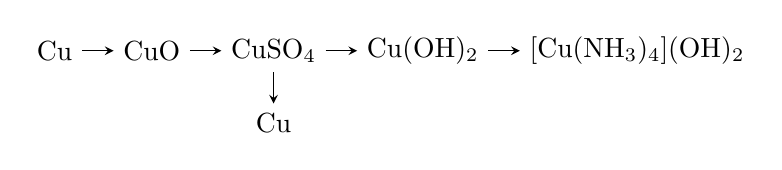
\begin{tikzpicture}[scale=1.0,>=stealth]
  \node (a) {\ce{Cu}};
  \node (b) [right =4mm of a] {\ce{CuO}};
  \node (c) [right =4mm of b] {\ce{CuSO4}};
  \node (d) [right =4mm of c] {\ce{Cu(OH)2}};
  \node (e) [below =4mm of c] {\ce{Cu}};
  \node (f) [right =4mm of d] {\ce{[Cu(NH3)4](OH)2}};
  \draw[->](a)--(b);
  \draw[->](b)--(c);
  \draw[->](c)--(d);
  \draw[->](c)--(e);
  \draw[->](d)--(f);
\end{tikzpicture}
\end{document}